%%%%%%%%%%%%%%%%%%%%%%%%%%%%%%%%%%%%%%%%%
% Beamer Presentation
% LaTeX Template
% Version 1.0 (10/11/12)
%
% This template has been downloaded from:
% http://www.LaTeXTemplates.com
%
% License:
% CC BY-NC-SA 3.0 (http://creativecommons.org/licenses/by-nc-sa/3.0/)
%
%%%%%%%%%%%%%%%%%%%%%%%%%%%%%%%%%%%%%%%%%

%----------------------------------------------------------------------------------------
%	PACKAGES AND THEMES
%----------------------------------------------------------------------------------------

\documentclass{beamer}

\mode<presentation> {

% The Beamer class comes with a number of default slide themes
% which change the colors and layouts of slides. Below this is a list
% of all the themes, uncomment each in turn to see what they look like.

%\usetheme{default}
%\usetheme{AnnArbor}
%\usetheme{Antibes}
%\usetheme{Bergen}
%\usetheme{Berkeley}
%\usetheme{Berlin}
\usetheme{Boadilla}
%\usetheme{CambridgeUS}
%\usetheme{Copenhagen}
%\usetheme{Darmstadt}
%\usetheme{Dresden}
%\usetheme{Frankfurt}
%\usetheme{Goettingen}
%\usetheme{Hannover}
%\usetheme{Ilmenau}
%\usetheme{JuanLesPins}
%\usetheme{Luebeck}
%\usetheme{Madrid}
%\usetheme{Malmoe}
%\usetheme{Marburg}
%\usetheme{Montpellier}
%\usetheme{PaloAlto}
%\usetheme{Pittsburgh}
%\usetheme{Rochester}
%\usetheme{Singapore}
%\usetheme{Szeged}
%\usetheme{Warsaw}

% As well as themes, the Beamer class has a number of color themes
% for any slide theme. Uncomment each of these in turn to see how it
% changes the colors of your current slide theme.

%\usecolortheme{albatross}
%\usecolortheme{beaver}
%\usecolortheme{beetle}
%\usecolortheme{crane}
%\usecolortheme{dolphin}
%\usecolortheme{dove}
%\usecolortheme{fly}
%\usecolortheme{lily}
%\usecolortheme{orchid}
%\usecolortheme{rose}
%\usecolortheme{seagull}
%\usecolortheme{seahorse}
%\usecolortheme{whale}
%\usecolortheme{wolverine}

%\setbeamertemplate{footline} % To remove the footer line in all slides uncomment this line
\setbeamertemplate{footline}[page number] % To replace the footer line in all slides with a simple slide count uncomment this line

%\setbeamertemplate{navigation symbols}{} % To remove the navigation symbols from the bottom of all slides uncomment this line
}
\usepackage{graphicx}
\usepackage{color}
\usepackage{soul}
\usepackage[mathstyleoff]{breqn}
\usepackage{gensymb}
\usepackage{braket}
\usepackage{mathtools}
\usepackage{caption}
\usepackage{subcaption}
\usepackage{multirow}
\usepackage{longtable}
\usepackage{booktabs}
\usepackage{placeins}
\usepackage{url}

\newcommand{\C}[1]{{\cal C}_{#1}}
\newcommand{\B}{{\cal B}}

\newcommand{\ac}[1]{{\color{blue} #1}}

\newcommand{\ord}{\mathcal{O}}
\newcommand{\nn}{\noindent}
\newcommand{\nb}{\nonumber}
\newcommand{\arccot}{{\rm arccot}}
\newcommand{\sss}{\scriptscriptstyle}
\newcommand{\dis}{\displaystyle}
\newcommand{\eq}[1]{\begin{equation} #1 \end{equation}}
\newcommand{\eqa}[1]{\begin{eqnarray} #1 \end{eqnarray}}
\newcommand{\Cc}[1]{{\cal C}_{#1}}
\newcommand{\Cp}[1]{{\cal C}_{#1}'}
\newcommand{\delC}[1]{\delta {\cal C}_{#1}}
\newcommand{\dC}[1]{{\cal C}_{#1}^{\rm NP}}
\newcommand{\dCp}[1]{{\cal C}_{#1^\prime}^{\rm NP}}
\newcommand{\av}[1]{\langle #1 \rangle}
\newcommand{\afb}{A_{\rm FB}}
\newcommand{\red}[1]{{\color{red} #1}}
\newcommand{\qm}[1]{{\color{blue} #1}}
\newcommand{\jv}[1]{{\red {#1}}}

\newcommand{\sect}[1]{\section{\hspace{-0.3cm} #1}}
\DeclareMathOperator{\Tr}{Tr}
\DeclarePairedDelimiter\abs{\lvert}{\rvert}%
% \midrule and \bottomrule in tables
\newcommand{\fluxunits}{ph \(\text{cm}^{-2} \text{ s}^{-1}\)}

%----------------------------------------------------------------------------------------
%	TITLE PAGE
%----------------------------------------------------------------------------------------

\title[Discovery of New Physics with ML]{Application of Machine Learning techniques to the discovery of new physics} % The short title appears at the bottom of every slide, the full title is only on the title page

\author{Óliver Partida Gutiérrez} % Your name
\institute[UAB] % Your institution as it will appear on the bottom of every slide, may be shorthand to save space
{
UAB \\ % Your institution for the title page
\medskip

}
\date{\today} % Date, can be changed to a custom date

\begin{document}

\begin{frame}
\titlepage % Print the title page as the first slide
\end{frame}

\begin{frame}
\frametitle{Outline} % Table of contents slide, comment this block out to remove it
\tableofcontents % Throughout your presentation, if you choose to use \section{} and \subsection{} commands, these will automatically be printed on this slide as an overview of your presentation
\end{frame}

%----------------------------------------------------------------------------------------
%	PRESENTATION SLIDES
%----------------------------------------------------------------------------------------

%------------------------------------------------
\section{Problem description} % Sections can be created in order to organize your presentation into discrete blocks, all sections and subsections are automatically printed in the table of contents as an overview of the talk
%------------------------------------------------

%\begin{frame}
%\frametitle{Paragraphs of Text}

%\end{frame}
%------------------------------------------------
%------------------------------------------------

%------------------------------------------------
%------------------------------------------------
\begin{frame}
\frametitle{Flavor-changing neutral currents FCNC }
\begin{columns}
	\begin{column}{0.5\textwidth}
	\begin{itemize}
		\item \(B\rightarrow K^*\mu\mu \)
		\item \(\Delta S = \Delta Q = \pm1 \).
		\item \(\Delta S = 2\) and FCNC only at second order in SM.
		\item Very suppressed processes by GIM mechanism.
		\item Candidates to search for new physics.
		
	\end{itemize}
	\end{column}
	\begin{column}{0.5\textwidth}  %%<--- here
		\begin{center}
		
				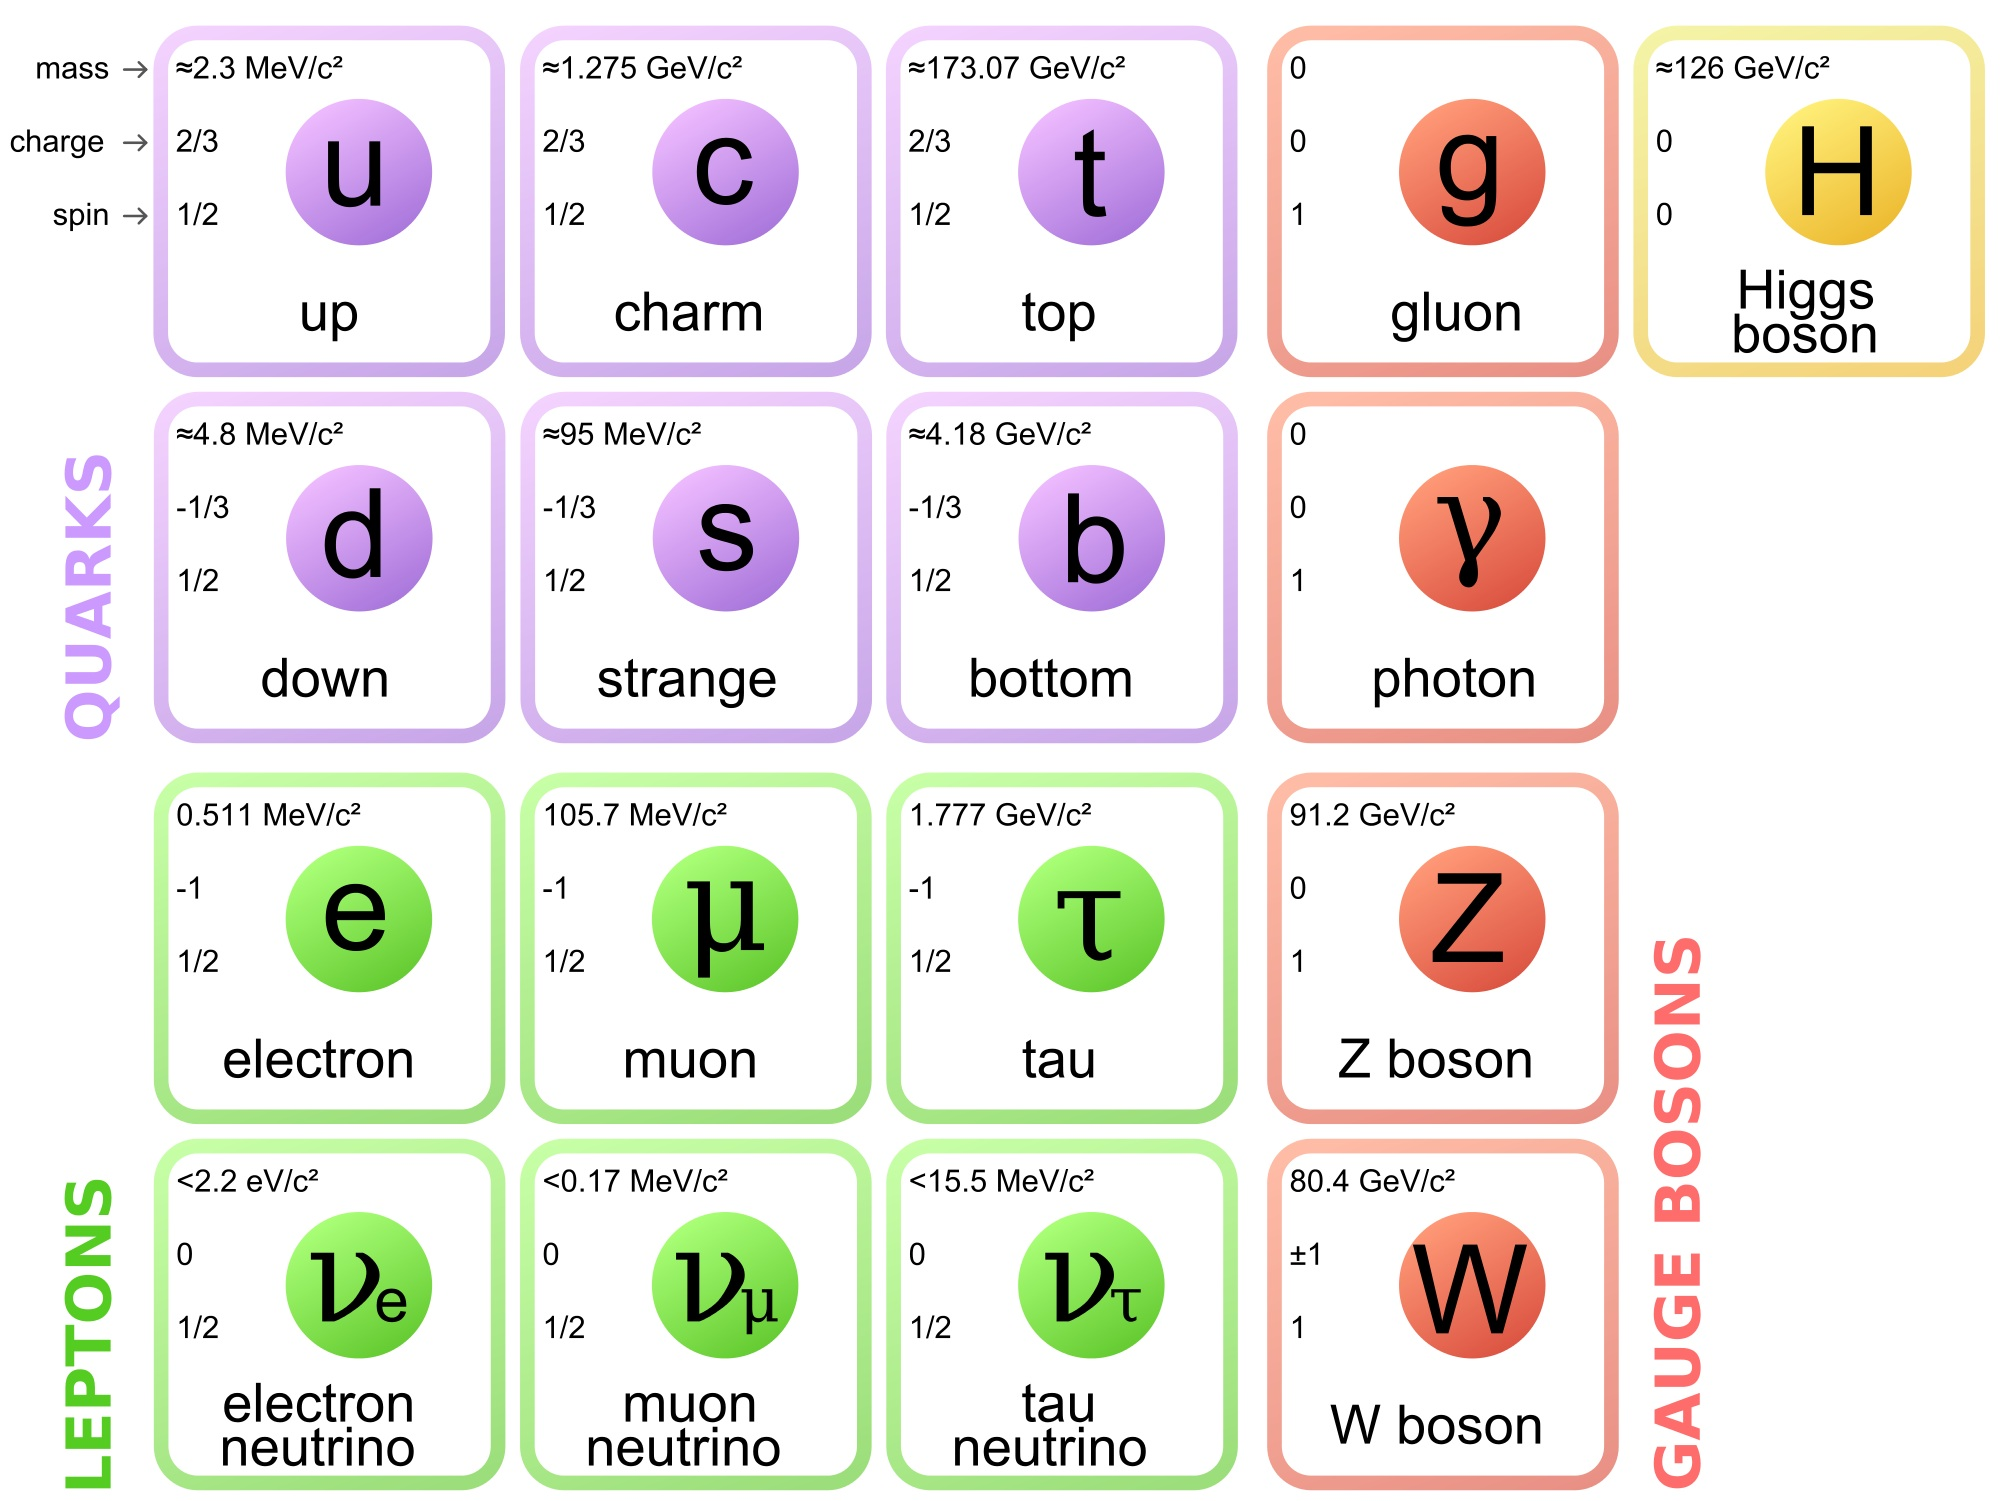
\includegraphics[width=1\textwidth, height=0.5\textheight]{imagenes/Standard_Model_of_Elementary_Particles.jpg}
				\label{fig:Standard Model}
		\end{center}
	\end{column}
\end{columns}


\end{frame}
\begin{frame}
\frametitle{GIM mechanism }
\begin{columns}
	\begin{column}{0.5\textwidth}
		\begin{itemize}
			\item Put forth by  Sheldon Lee Glashow, John Iliopoulos and Luciano Maiani.
			\item Required the introduction of a new quark.
			\item  mass-squared difference of the different virtual quarks exchanged in the box diagram.
			
		\end{itemize}
	\end{column}
	\begin{column}{0.5\textwidth}  %%<--- here
		\begin{center}			
			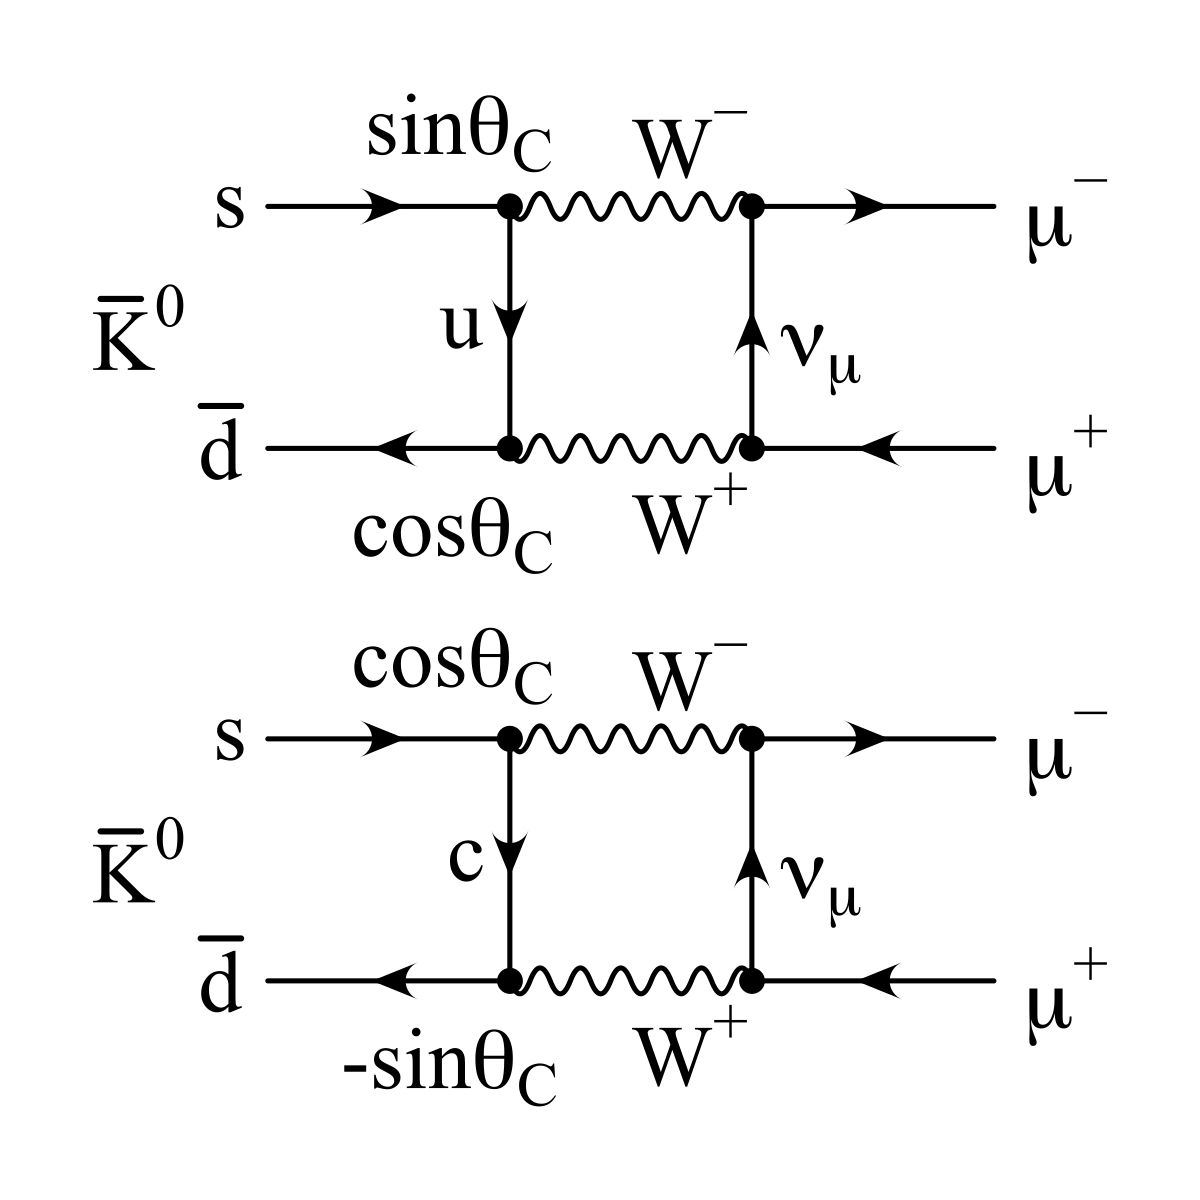
\includegraphics[width=1\textwidth, height=.6\textheight]{imagenes/Gim.png}
			\captionof{figure}\textbf{Neutral Kaon decay}
			 \cite{GIMMechanism}
			\label{fig:GIM}
		\end{center}
	\end{column}
\end{columns}

\end{frame}
\begin{frame}
\frametitle{Experimental data }
\begin{itemize}
	\item In 2013,
	the LHCb collaboration announced the measurement of angular observables describing
	the decay \(B \rightarrow K^∗\mu\mu \).
	\item Two observables, \(P_2 \) and \(P^{\prime}_5\) were in significant disagreement with the SM expectations.
	\item \(RK = Br(B \rightarrow K\mu\mu)/Br(B \rightarrow Kee) \) measurement $\neq$ 1. Could indicate Lepton Flavor Universality Violation (LFUV).
\end{itemize}
\begin{figure}
	\centering
	\begin{minipage}{.5\textwidth}
		\centering
		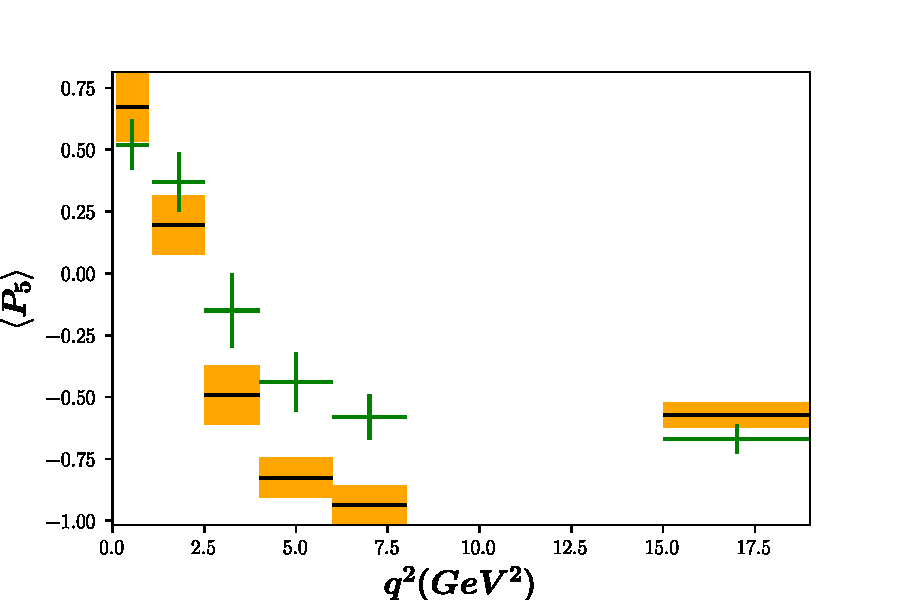
\includegraphics[width=.8\linewidth]{imagenes/P5.pdf}
		\caption{Observable \(P_5\).}
		\label{fig:P5}
	\end{minipage}%
	\begin{minipage}{.5\textwidth}
		\centering
		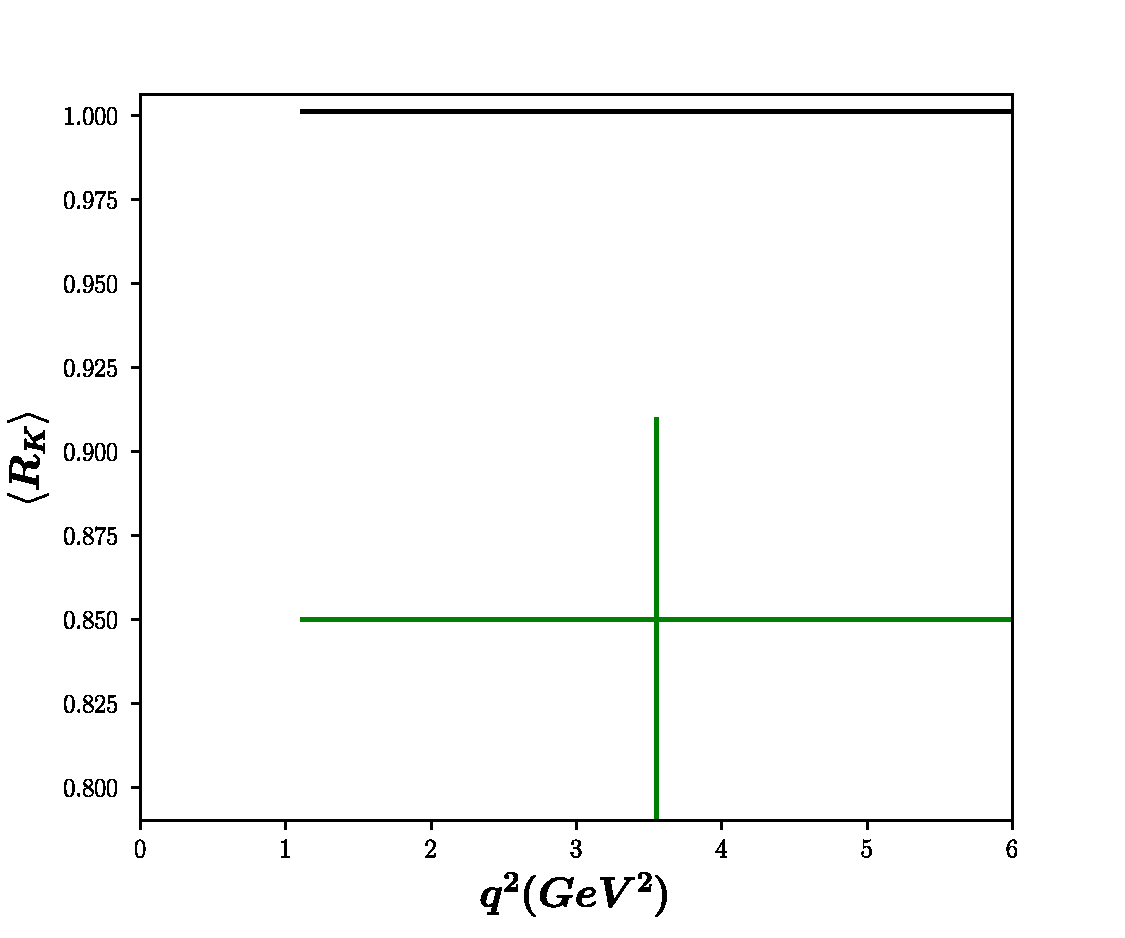
\includegraphics[width=.8\linewidth]{imagenes/RK.pdf}
		\caption{\(R_K = Br(B\rightarrow K\mu\mu)/ Br(B\rightarrow Kee)\).}
		\label{fig:RK}
	\end{minipage}
\end{figure}



\end{frame}

\begin{frame}
\frametitle{Searching for New Physics}
\begin{itemize}
	\item Effective field theory framework (EFT)
\end{itemize}

\[
\mathcal{H}_{eff} = -\frac{4G_F}{\sqrt{2}}V_{tb}V^*_{ts}\sum_{i}\mathcal{C}_i\mathcal{O}_i.
\]

 \begin{itemize}
 	\item  Heavy degrees of freedom (the top quark, the \(W\) and \(Z\) bosons, the Higgs and any heavy new particle) are integrated out in short-distance Wilson coefficients \( \mathcal{C}_i \), leaving only a set of operators \(\mathcal{O}_i \) describing the physics at long distances.
 	\item In the SM, the Hamiltonian contains 10 main operators with specific chiralities due to the V - A structure
 	of the weak interactions.
 	\item We reduce such set to the two dominant operators:
 	%\[
 	%\mathcal{O}_7 = %\frac{e}{16\pi^2}m_b(\bar{s}\sigma_{\mu\nu}P_Rb)F^{\mu\nu},
 	%\]
 	\[
 	\mathcal{O}_9 = \frac{e}{16\pi^2}m_b(\bar{s}\gamma_{\mu}P_Lb)(\bar{\ell}\gamma^{\mu}\ell),
 	\]
 	\[
 	\mathcal{O}_{10} = \frac{e}{16\pi^2}m_b(\bar{s}\gamma_{\mu}P_Lb)(\bar{\ell}\gamma^{\mu}\gamma_{5}\ell).
 	\]

 \end{itemize}



\end{frame}

\begin{frame}
\frametitle{Searching for New Physics}
\begin{itemize}
	\item Current analysis of anomalies in 
flavor physics are based on a linear regression of a \(\chi^2 \) function.
	\item The observables measured by the experimental collaborations can be written in
	terms of the \(C_i \)  Wilson coefficients.
	\item It is common to split the Wilson coefficients
	in two pieces: the SM contributions and the NP contributions:
	\[
	C_9 = C^{SM}_9 + C^{NP}_9
	\]
	\[
	C_{10} = C^{SM}_{10} + C^{NP}_{10}
	\]
\end{itemize}
 


\end{frame}
\section{Machine Learning techniques}
%------------------------------------------------
%------------------------------------------------
%------------------------------------------------
\begin{frame}
\frametitle{Discriminative vs Generative}
\begin{itemize}
\item Two distinct approaches to solving decision problems.
\item Generative:
\begin{itemize}
\item Determine the class-conditional densities \(p(x|C_k) \) for each class individually
and the prior class probabilities.
\item Use Bayes theorem to find the posterior:
\[
p(C_k|x) = \frac{p(x|C_k)p(C_k)}{p(x)}
\]
\item We have a model of our data. We can sample from it.
\item E.g.: Naive Bayes, Mixture Models, Generative Adversarial Networks.
\end{itemize}
\item Discriminative:
\begin{itemize}
	\item We have labeled data.
	\item Directly determine the posterior class probabilities \(p(C_k|x)\).
	\item E.g.: Neural Networks.
\end{itemize}
	
\end{itemize}

\end{frame}
%------------------------------------------------
%------------------------------------------------
%------------------------------------------------
%------------------------------------------------

\begin{frame}
\frametitle{Generative models}
\begin{itemize}
	\item \(p(x|\mu,\Sigma,\pi) = \sum_{i=1}^{k}\pi_i p(x|\mu_i,\Sigma_i) \).
		\item Model the probability distribution of the data.
	\item Fit model parameters using Maximum Likelihood.
	\item Use Bayes theorem to classify new data point.

\end{itemize}

\begin{figure}
	\centering
	\begin{minipage}{.5\textwidth}
		\centering
		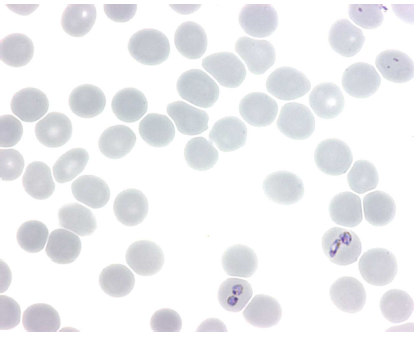
\includegraphics[width=.8\linewidth]{imagenes/malaria.png}
	
		\label{fig:malaria}
	\end{minipage}%
	\begin{minipage}{.5\textwidth}
		\centering
		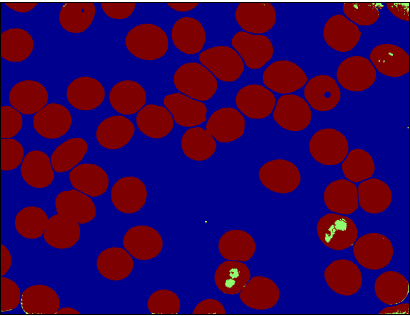
\includegraphics[width=.8\linewidth]{imagenes/MalariaSegmented.png}
		
		\label{fig:malariasegmented}
	\end{minipage}
\end{figure}



\end{frame}

%------------------------------------------------
%------------------------------------------------
%------------------------------------------------
%------------------------------------------------
\begin{frame}
\frametitle{Generative Adversarial Networks (GANs)}
\begin{itemize}
	\item First described in the 2014 paper by Ian Goodfellow \cite{goodfellow2014generative}.
	\item  \textbf{What are they?} $\rightarrow$ Model architecture for training a generative model.
	\item Implicitly learn rich distributions hard to model with an explicit likelihood.
	
	
	
\end{itemize}
\begin{figure}
	\centering
	\begin{minipage}{1\textwidth}
		\centering
		\includegraphics[width=.8\textwidth]{imagenes/gan.png}
		\captionof{figure}{\textbf{GAN architecture}, from Recent Progress on Generative Adversarial Networks (GANs): A Survey \cite{ZhaoqingPan}}
		\label{fig:GANArchitecture}
	\end{minipage}%
	
\end{figure}



\end{frame}
%------------------------------------------------
%------------------------------------------------
%------------------------------------------------
\begin{frame}
\frametitle{GAN training problems}

\begin{itemize}
	\item \textbf{Vanishing gradients} $\rightarrow$ optimal discriminator doesn't provide enough information for the generator to make progress.
	\item \textbf{Mode collapse} $\rightarrow$  if a generator produces an especially plausible output, the generator may learn to produce only that output.
	\item \textbf{Failure to converge} $\rightarrow$  If the generator succeeds perfectly, then the discriminator has a 50\% accuracy and the discriminator feedback gets less meaningful over time.
\end{itemize}
\begin{figure}

\end{figure}

\end{frame}
%------------------------------------------------
%------------------------------------------------
%------------------------------------------------

\section{Results}

%------------------------------------------------



%------------------------------------------------

%------------------------------------------------
%------------------------------------------------
%------------------------------------------------
%------------------------------------------------
\begin{frame}
\frametitle{Results. Dataset}
\begin{itemize}
	\item 8 observables.
	\item 37 bin values.
	\item 10000 samples. 
	\item \(10 \times 10\) \(C_9 \in [-2, 0] \),  \(C_{10} \in [-1, 1]. \)
	\item \(100\) \(a_0, a_1, a_2 \in [-0.01, 0.01]. \)
\end{itemize}
\begin{table}
	\begin{tabular}{ |c|c|c|c|  } 
		\hline
		\small
		\(C_9 = -1.33\), \(C_{10} = -0.44\)  \(\chi^2 = 23.33 \)\normalsize
		& \textbf{\(a_0\)} & \textbf{\(a_1\)} & \textbf{\(a_2\)}\\
		\hline
		\(P_1\) & -0.093  & 0.001 &  0 \\
		\hline
		\(P_2\) & -0.093  & 0.001 &  0 \\
		\hline
		\(P_4\) & -0.093  & 0.001 &  0 \\
		\hline
		\(P_5\) & -0.093  & 0.001 &  0 \\		
		\hline
		\(BrK^{0*}\) & -0.093  & 0.001 &  0 \\	
		\hline
		\(BrK^{0}\) & -0.093  & 0.001 &  0 \\		
		\hline	
		\(R_{K}\) & -0.093  & 0.001 &  0 \\
		\hline	
		\(R_{K^*}\) & -0.093  & 0.001 &  0 \\	
		\hline
	\end{tabular}
	\caption{\label{tab:GANExp3BestSample} Coefficients of sample in training set with lowest \(\chi^2 \) value.}
\end{table}
\end{frame}
\begin{frame}

\frametitle{Results. Neural networks}

	\begin{table}
		\begin{tabular}{ |c|c|c|c|  } 
			\hline
			\small
			\(C_9 = -0.79\), \(C_{10} = -0.07\),  \(\chi^2 = 29.5 \)\normalsize
			& \textbf{\(a_0\)} & \textbf{\(a_1\)} & \textbf{\(a_2\)}\\
			\hline
			\(P_1\) & 0 & 0 &  0 \\
			\hline
			\(P_2\) & 0 & 0 & 0 \\	
			\hline
			\(P_4\) & 0.03 & 0 &	0 \\
			\hline
			\(P_5\) & 0.02 &   0 &   0 \\		
			\hline
			\(BrK^{0*}\) & -0.01 & 0 & 0 \\		
			\hline
			\(BrK^{0}\) & -0.01 & 0 & 0 \\		
			\hline	
			\(R_{K}\) & -0.01 & 0 & 0 \\
			\hline	
			\(R_{K^*}\) & -0.01 & 0 & 0 \\		
			\hline
		\end{tabular}
		\caption{\label{tab:NNExp2NNPrediction} Coefficients predicted by the NN after training}
	\end{table}
\end{frame}
\begin{frame}
\frametitle{Results. GAN}
\begin{table}
	\begin{tabular}{ |c|c|c|c|  } 
		\hline
		\small
		\(C_9 = -0.74\), \(C_{10} = -0.62\) ,  \(\chi^2 = 373.48 \)
		\normalsize
		& \textbf{\(a_0\)} & \textbf{\(a_1\)} & \textbf{\(a_2\)}\\
		\hline
		\(P_1\) & 0.012 & 0.016 &  0.0008 \\
		\hline
		\(P_2\) & -0.017 & 0.030 & -0.002 \\	
		\hline
		\(P_4\) & -0.010 & 0.010 &	-0.001 \\
		\hline
		\(P_5\) & 0.001 &  0.008 &   0.0003 \\		
		\hline
		\(BrK^{0*}\) & -0.026 & 0.023 & 0.001 \\		
		\hline
		\(BrK^{0}\) & -0.008 & 0.014 & 0.005 \\		
		\hline	
		\(R_{K}\) & -0.019 & 0.012 & -0.004 \\
		\hline	
		\(R_{K^*}\) & -0.013 & 0.011 & -0.006 \\		
		\hline
		
		
	\end{tabular}
	\caption{\label{tab:GAN3Results} Coefficients with lowest \(\chi^2 \) sampled from GAN. }
\end{table}
\end{frame}

\section{Conclusions}

\begin{frame}
\frametitle{Conclusions}
\begin{itemize}
\item The parametrization of the observables
\end{itemize}
\end{frame}

%------------------------------------------------




%------------------------------------------------

\begin{frame}
\Huge{\centerline{Thank you}}
\end{frame}

\begin{thebibliography}{99}
	
	%\cite{Alguero:2019ptt}
	\bibitem{Alguero:2019ptt}
	M.~Alguer\'o, B.~Capdevila, A.~Crivellin, S.~Descotes-Genon, P.~Masjuan, J.~Matias, M.~Novoa and J.~Virto,
	%``Emerging patterns of New Physics with and without Lepton Flavour Universal contributions,''
	Eur. Phys. J. C \textbf{79} (2019) no.8, 714
	%doi:10.1140/epjc/s10052-019-7216-3
	[arXiv:1903.09578 [hep-ph]].
	%82 citations counted in INSPIRE as of 17 Apr 2020
	
	\bibitem{Alguero:2018nvb}
	M.~Alguer\'o, B.~Capdevila, S.~Descotes-Genon, P.~Masjuan and J.~Matias,
	%``Are we overlooking lepton flavour universal new physics in $b\to s\ell\ell$ ?,''
	Phys.\ Rev.\ D {\bf 99} (2019) no.7,  075017
	%doi:10.1103/PhysRevD.99.075017
	[arXiv:1809.08447 [hep-ph]].
	%%CITATION = doi:10.1103/PhysRevD.99.075017;%%
	
	%\cite{Vicente:2020usa}
	\bibitem{Vicente:2020usa}
	A.~Vicente,
	%``Theory status and implications of $R_K^{(\ast)}$,''
	[arXiv:2001.04788 [hep-ph]].
	%1 citations counted in INSPIRE as of 17 Apr 2020
	
	\bibitem{Aaij:2019wad}
	R.~Aaij {\it et al.} [LHCb Collaboration],
	% ``Search for lepton-universality violation in $B^+\to K^+\ell^+\ell^-$ decays,''
	arXiv:1903.09252 [hep-ex].
	%%CITATION = ARXIV:1903.09252;%%
	
	\bibitem{BelleRK}
	S.~Choudhury for the Belle collaboration, ``Measurement of Lepton Flavour Universality in $B$ decays at Belle'', Talk at `EPS-HEP Conference 2019'.
	
	\bibitem{Aaij:2014pli}
	R.~Aaij {\it et al.} [LHCb Collaboration],
	% ``Differential branching fractions and isospin asymmetries of $B \to K^{(*)} \mu^+ \mu^-$ decays,''
	JHEP {\bf 1406} (2014) 133
	% doi:10.1007/JHEP06(2014)133
	[arXiv:1403.8044 [hep-ex]].
	%%CITATION = doi:10.1007/JHEP06(2014)133;%%
	
	
	\bibitem{Abdesselam:2019wac}
	A.~Abdesselam {\it et al.} [Belle Collaboration],
	%``Test of lepton flavor universality in ${B\to K^\ast\ell^+\ell^-}$ decays at Belle,''
	arXiv:1904.02440 [hep-ex].
	%%CITATION = ARXIV:1904.02440;%%
	
	\bibitem{Aaboud:2018mst}
	M.~Aaboud {\it et al.} [ATLAS Collaboration],
	% ``Study of the rare decays of $B^0_s$ and $B^0$ mesons into muon pairs using data collected during 2015 and 2016 with the ATLAS detector,''
	%Submitted to: JHEP
	[arXiv:1812.03017 [hep-ex]].
	%%CITATION = ARXIV:1812.03017;%%
	
	\bibitem{FLAG}
	S.~Aoki {\it et al.} [Flavour Lattice Averaging Group],
	% ``FLAG Review 2019,''
	arXiv:1902.08191 [hep-lat].
	%%CITATION = ARXIV:1902.08191;%%
	
	\bibitem{Wehle:2016yoi}
	S.~Wehle {\it et al.} [Belle Collaboration],
	%``Lepton-Flavor-Dependent Angular Analysis of $B\to K^\ast \ell^+\ell^-$,''
	Phys.\ Rev.\ Lett.\  {\bf 118} (2017) no.11,  111801
	%  doi:10.1103/PhysRevLett.118.111801
	[arXiv:1612.05014 [hep-ex]].
	%%CITATION = doi:10.1103/PhysRevLett.118.111801;%%
	%195 citations counted in INSPIRE as of 25 Apr 2019
	
	
	\bibitem{Abdesselam:2016llu}
	A.~Abdesselam {\it et al.} [Belle Collaboration],
	%``Angular analysis of $B^0 \to K^\ast(892)^0 \ell^+ \ell^-$,''
	arXiv:1604.04042 [hep-ex].
	%%CITATION = ARXIV:1604.04042;%%
	%139 citations counted in INSPIRE as of 25 Apr 2019
	
	\bibitem{Calibbi:2017qbu}
	L.~Calibbi, A.~Crivellin and T.~Li,
	% ``Model of vector leptoquarks in view of the $B$-physics anomalies,''
	Phys.\ Rev.\ D {\bf 98} (2018) no.11,  115002
	% doi:10.1103/PhysRevD.98.115002
	[arXiv:1709.00692 [hep-ph]].
	%%CITATION = doi:10.1103/PhysRevD.98.115002;%%
	
	
	\bibitem{Crivellin:2019dun}
	A.~Crivellin, D.~Muller and C.~Wiegand,
	% ``$b\to s\ell^+\ell^-$ Transitions in Two-Higgs-Doublet Models,''
	arXiv:1903.10440 [hep-ph].
	%%CITATION = ARXIV:1903.10440;%%
	
	\bibitem{Bobeth:2016llm}
	C.~Bobeth, A.~J.~Buras, A.~Celis and M.~Jung,
	%``Patterns of Flavour Violation in Models with Vector-Like Quarks,''
	JHEP {\bf 1704} (2017) 079
	%doi:10.1007/JHEP04(2017)079
	[arXiv:1609.04783 [hep-ph]].
	%%CITATION = doi:10.1007/JHEP04(2017)079;%%
	\bibitem{ZhaoqingPan}
	Z. Pan, W. Yu, X. Yi, A. Khan, F. Yuan and Y. Zheng, "Recent Progress on Generative Adversarial Networks (GANs): A Survey," in IEEE Access, vol. 7, pp. 36322-36333, 2019, doi: 10.1109/ACCESS.2019.2905015.
	\bibitem{goodfellow2014generative}
	Ian J. Goodfellow and Jean Pouget-Abadie and Mehdi Mirza and Bing Xu and David Warde-Farley and Sherjil Ozair and Aaron Courville and Yoshua Bengio
	[arXiv:1406.2661 [stat.ML]].
	\bibitem{GIMMechanism} 
	GIM mechanism --- {Wikipedia}{,} The Free Encyclopedia,
	\\\texttt{\url{https://en.wikipedia.org/w/index.php?title=GIM_mechanism&oldid=958923133}}
	


	
	
\end{thebibliography}
\end{document} 